\section{Backend}
Als Technologie für die Implementierung des Backends wird das Asp.Net Core Framework von Microsoft eingesetzt. Grund dafür ist, dass alle benötigten Funktionen wie Webfrontends, REST APIs oder Identity Management nativ und gleichzeitig plattformunabhängig unterstützt werden. Als Programmiersprache wird C\# eingesetzt.

\subsection{Authentifizierung und Autorisierung}
Für die Umsetzung der Benutzerauthentifizierung und die Rechteverwaltung wird IdentityServer4\cite{Allen2016} eingesetzt. Dieses Framework erlaubt eine moderne zentralisierte Identitätsverwaltung für verschiedene Anwendungsszenarien basierend auf OpenId und OAuth2. 

\begin{figure}[h]
  \begin{center}
    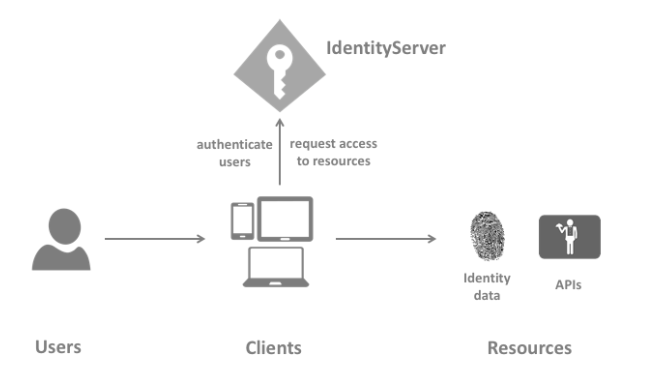
\includegraphics[width=\textwidth]{./img/BackendIdentityServer.png}
    \caption{Terminologien des Identity Servers}
    \label{fig:backendIdentityServer}
  \end{center}
\end{figure}

Das Grundkonzept des Identity Servers wird in Abbildung \ref{fig:backendIdentityServer} gezeigt. \textbf{Benutzer} greifen dabei über verschiedene \textbf{Clients} auf geschützte \textbf{Ressourcen} wie APIs oder Anwendungsbereiche zu, die von dem Identitätsserver geschützt werden. Dieses Konzept passt auf das in diesem Projekt entstehende Szenario, in dem Benutzer entweder über die Smartphone App oder das Webfrontend des Backends (Clients) auf die Web API zugreifen (Ressource).

\begin{figure}[h]
  \begin{center}
    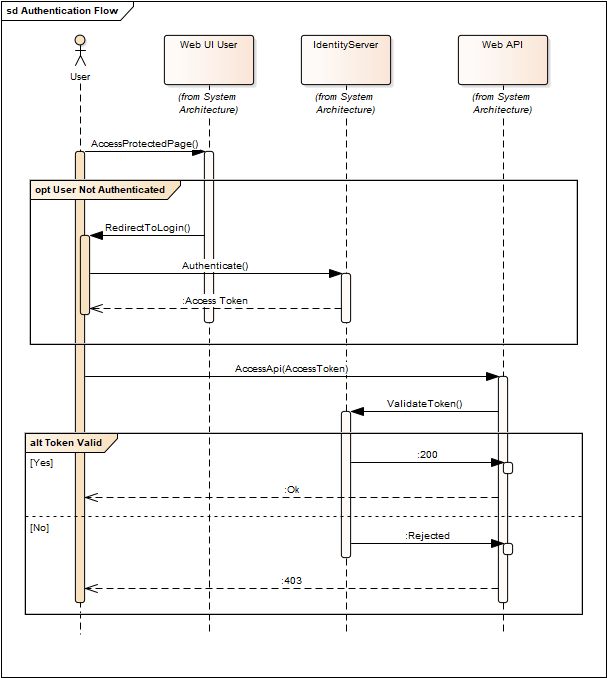
\includegraphics[width=\textwidth]{./img/BackendAuthenticationFlow.png}
    \caption{Ablauf der Authentifizierung beim Zugriff auf geschützte Ressourcen}
    \label{fig:backendAuthenticationFlow}
  \end{center}
\end{figure}

Der implementierte Ablauf der Authentifizierung erfolgt nach dem in Abbildung \ref{fig:backendAuthenticationFlow} skizzierten Schema. Beim Zugriff auf eine geschützte Funktion im Web UI wird der Benutzer auf die Login Seite des Identity Servers weitergeleitet, wo er sich entweder registrieren oder einloggen kann. Nach erfolgreicher Authentifizierung generiert der Identity Server ein Access Token, welches in der Session des Benutzers gespeichert wird und Informationen über den Benutzer, die für ihn freigegebenen Ressourcen sowie die dem Nutzer zugeordneten Claims enthält. Bei einem anschließenden Zugriff die Web API wird dieses Token mitgeschickt und von der API beim Identity Server validiert.

\subsection{Datenbank und Zugriff}
Als Datenbank wird MySql eingesetzt da es einfach in der Anwendung und schlank im Betrieb ist. Als alternative wurde ebenfalls Sql Server evaluiert, was den Vorteil der besseren Integration in die Asp.Net Core Umgebung gehabt hätte. Der zugehörige Docker Container (vgl. \ref{sec:backendDeployment}) hat jedoch 4GB Arbeitsspeicher erfordert, was zusätzlich zum normalen Betriebssystem und der Entwicklungsumgebung mehr als die momentan üblicherweise verbauten 8GB \ac{RAM} übertrifft.\todo{Weshalb es auf unseren Systemen nicht getestet werden konnte - vllt ergänzen}

Der Zugriff auf die Datenbank erfolgt nicht direkt über SQL-Anfragen sondern über Entity Framework, ein Framework für objektrelationale Abbildung. Dabei werden die Daten im Hintergrund in Collections geladen, sodass es für den Benutzer aussieht, als würden die Daten direkt im RAM liegen. Dieses System bietet - insbesondere in Kombination mit \ac{LINQ} in C\#- den Vorteil, dass der Code wesentlich übersichtlicher und leichter verständlich wird, da das direkte Laden der Daten mittels SQL-Anfragen und anschließendem manuellen Einlesen entfällt.

Für die Integration von Entity Framework für MySql Datenbanken in einer Asp.Net Core Umgebung muss ein Third Party NuGet Paket\cite{Microsoft2018} verwendet werden, da zum Zeitpunkt der Entwicklung keine native Anbindung zur Verfügung steht. Das verwendete Paket hat allerdings Performanceprobleme bei der Verarbeitung größerer Datenmengen. Schon das Speichern und Laden von Fahrten mit einer Rohdatenmenge von ~500kB führen zu Verzögerungen von ca. 30 Sekunden. Die einzig verbleibende Alternative um das Problem zu beheben ist der Austausch der Datenbank, wozu während der Projektlaufzeit keine Ressourcen mehr zur Verfügung stehen.

\subsection{Bereitstellung}
\label{sec:backendDeployment}
Da das Backend aus verschiedenen zunächst unabhängigen Komponenten besteht und einige Voraussetzungen bezüglich der Infrastruktur mit sich bringt, ist die Bereitstellung einer Produktivumgebung nicht trivial. 
Aus diesem Grund wird die Containervirtualisierung Docker eingesetzt, um das Gesamtsystem leicht installierbar zu machen.

Docker\cite{Inc.2018} unterscheidet von normalen virtuellen Maschinen darin, dass nicht für jede Instanz ein gesamtes Hostsystem emuliert wird, sonder lediglich die Applikation samt ihrer Abhängigkeiten in dem Container stecken. In der Terminologie wird bei Docker zwischen Containern und Images unterschieden. Ein Image ist dabei ein Speicherabbild, aus dem heraus sich mehrere Container starten lassen (vergleichbar mit Klassen und Instanzen bei objektorientierter Programmierung). Für die Installation bedeutet das, dass nur die Images aller am System beteiligten Module zur Verfügung stehen müssen um aus jedem Image einen Container zu starten. Um das hochfahren komplexerer Anwendungen, die aus mehreren Containern bestehen, zu erleichtern, gibt es das Tool Docker Compose. Hiermit lassen sich verschiedene Parameter einstellen und alle Container gemeinsam starten was den Aufwand bei der Bereitstellung weiter reduziert. 

Um das SmartCar Backend in einer neuen Umgebung auszurollen werden lediglich die Images der Module, sowie das docker-compose File benötigt. Zusätzlich muss natürlich Docker auf dem Zielsystem installiert sein. Ist alles vorhanden, lässt sich über den Befehl \texttt{docker-compose up} die gesamte Umgebung ohne zusätzliche Installationen hochfahren.

\subsection{Datenanalyse am Beispiel Kraftstoffverbrauch}
Wie bei \ref{Sec_AnayseDerAufgezeichnetenDaten} beschrieben ist, war es von Anfang an ein Ziel die Daten nicht nur zu sammeln, sondern auf diesen anschließend Analysen auszuführen um dem Fahrer somit einen zugewinne an Informationen zu ermöglichen. 

Eine dieser Analysen ist die Ermittlung des Kraftstoffverbrauch. Aktuelle Autos stellen diese Information dem Fahrer inzwischen zwar meist per Bordcomputer zur Verfügung, Fahrer älterer Fahrzeuge erhalten diese Informationen jedoch nicht. Weiterhin könnte bei der Berücksichtigung des \enquote{Dieselskandals} aus jüngster Zeit auch die Frage aufkommen, ob die angezeigten Informationen überhaupt der Realität entsprechen, da ja bereits die Herstellerangaben im täglichen Betrieb äußerst selten eingehalten werden können.

Um eine solche Analyse durchführen zu können, müssen zuerst die benötigten Informationen aus dem Track extrahiert werden:\newline
Da die Datenbank Anbindung (siehe xy \todo{referenz auf datenbank performance problem beschreibung}) das \enquote{bottelneck} des Backends darstellt, wurde um dieses möglichst wenig zu belasten keine generischen Funktionen geschrieben um die zur Berechnung benötigten Daten aus den Traces extrahieren, sondern für jede Analyse eine eigene. In diesen werden die Daten eines Traces durchlaufen und bei Übereinstimmung der \acs{PID} mit den ausgewählten \acp{PID} extrahiert.

Für aktuelle Autos ist es mit den gemessenen Verbrauchswerten anschließend möglich einen Kraftstoffverbrauch zu bestimmen bzw. diesen gegenüber z.B. der Geschwindigkeit in einem Diagramm anzuzeigen.

Bei älteren Autos, welche nicht messen wie viel Kraftstoff verbraucht wird oder diese Informationen nicht ober \ac{OBD} zu Verfügung stellen ist die Analyse komplexer. Aus diesem Grund gibt es auch mehrere wissenschaftliche Arbeiten die sich in diesem Zusammenhang auch mit der \ac{OBD} Schnittstelle beschäftigen \todo{Hier fehlen noch die Referenzen aus michis text [2][3]}. Der Konsens dieser Arbeiten ist, dass sich der Momentanverbrauch, sofern er sich nicht über die \ac{PID} 0x5E auslesen lässt, mithilfe anderer Berechnen lässt.
Dazu wird im Grunde die Formel \ref{GrundFormelMomentanVerbrauch} verwendet. 

Die Konstante $AirFuelRatio_\text{Stöch}$ gibt das Verhältnis von Luft und Kraftstoff an, bei der alle
Kohlenwasserstoff-Moleküle mit allen Sauerstoffmolekülen der angesaugten Luft reagieren. Dieses
Verhältnis ist für den Verbrennungsvorgang optimal, und beträgt bei Ottomotoren 14,7 und bei
Dieselmotoren 14,5.

\begin{equation}
\label{GrundFormelMomentanVerbrauch}
Sprit(\frac{g}{sec}) = \frac{Luftmasse(\frac{g}{sec})}{\lambda*AirFuelRatio_\text{Stöch}}
\end{equation}

Mit Formel \ref{GrundFormelMomentanVerbrauch} kann nun anhand der Dichte auf den Momentanverbrauch in Litern geschlossen werden. Dazu verwendet man Formel \ref{DichteZuVerbrauchInLiter}. Dabei ist $\rho$ die gemittelte Dichte des Kraftstoffs. Für Ottokraftstoff beträgt diese etwa 747,5
Gramm pro Liter, für Diesel dagegen etwa 832,5 Gramm pro Liter\cite{Aral2018}. 

\begin{equation}
\label{DichteZuVerbrauchInLiter}
Sprit(\frac{l}{sec}) = \frac{Sprit(\frac{g}{sec})}{\rho}
\end{equation}
 
Für die Berechnung wird als nächstes $\lambda$ benötigt. Hierbei handelt es sich um das gemessene Luft-Treibstoff-Verhältnis, welches über eine Lambda-Sonde gemessen wurde. DDieser Wert kann laut ISO 15031-5 mit Formel \ref{FormelFuerLambda} berechnet werden.

\begin{equation}
\label{FormelFuerLambda}
EQRAT 11_\text{PID 24}=DATAab_{(\text{PID 24})}*(\frac{DATAa_{(\text{PID 4F})}}{65535})
\end{equation}

$DATAab_{\text{PID 24}}$ entspricht hierbei dem Sensorwert, welcher über die ersten beiden Bytes der \ac{PID} 0x24 ausgelesen wird (alternativ können je nach Verfügbarkeit auch die \acp{PID}) 0x25-0x2B oder 0x34-0x3B verwendet werden).
\newline
$DATAa_{(\text{PID 4F})}$ gibt die Skalierung an.
\newline
Sollten die \acp{PID}) 0x24-0x2B oder 0x34-0x3B nicht verfügbar sein, gibt es auf hierfür weitere Möglichkeiten zur Berechnung, diese benötigen jedoch immer spezifischere Daten für das Verwendete Auto und wurden deshalb mangelns fehlender Messtechnik nicht weiter implementiert.

Als letztes wird für die Berechnung noch der Luftfluss benötigt. Dieser lässt sich im einfachsten Fall mithilfe der \ac{PID} 0x10 ermitteln und anschließend durch den zugehörigen Korrekturfaktors \ac{PID} 0x50 korrigieren.

Für den Fall, dass der Wert des Luftmassesensors nicht abrufbar ist, so wurde in \todo{hier fehlt auch noch referenz auf [3] aus michs text} eine Möglichkeit vorgestellt, wie sich dieser Wert mithilfe der Werte der EngineLoad (\ac{PID} 0x04) und der Motordrehzahl (\ac{PID} 0x0C0) ermitteln lässt. Jedoch werden auch für diese Berechnung spezifische Messdaten für das zugehörige Auto benötigt welche meist nicht vorliegen.

 
 
 
 
